\chapter{Proposta do trabalho} \label{cap:proposta}

Conforme descrito no Capítulo \ref{cap:introducao}, este trabalho será constituído de cinco etapas.
Em um primeiro momento, a etapa de diagnóstico foi realizada e os sistemas relacionados e suas funcionalidades em comum 
foram apresentadas no Capítulo \ref{cap:sistemas_relacionados}. Neste capítulo é apresentado o resultado da segunda etapa
que é a descrição da proposta do trabalho de acordo com os objetivos estabelecidos.

Para a plataforma ``Empurrando Juntos'' o lado servidor da arquitetura definida é denominado Pentano e pode ser visualizado na Figura \ref{fig:pentano}. 
O Pentano é constituído por dois módulos: o \textit{server}, 
que é o módulo da API a ser criada neste trabalho e o \textit{Math} que é o módulo responsável pela clusterização. 

\begin{figure}[h!]
\centering
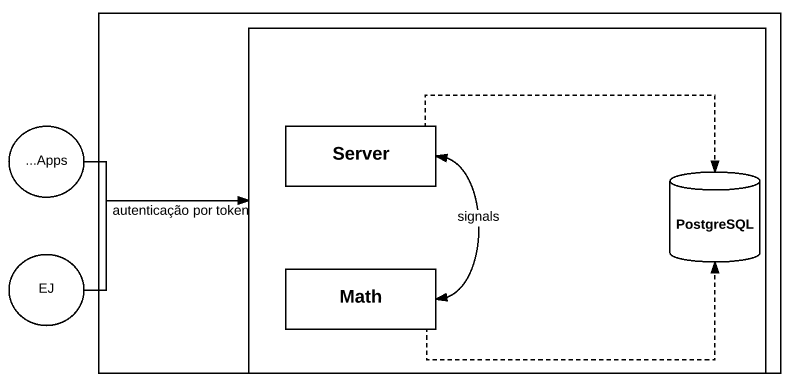
\includegraphics[scale=0.8]{figuras/esquema_pentano.png}
\caption{Estrutura do Pentano}
\label{fig:pentano}
\end{figure}

\section{Requisitos da solução} \label{sec:requisitos}

Uma avaliação do escopo da plataforma ``Empurrando Juntos'' permitiu o levantamento de características do sistema e por consequência
os requisitos associados, que foram sumarizados na Tabela \ref{tab:requisitos}.

\begin{table}[h!]
\centering
\caption{Requisitos da aplicação}
\label{tab:requisitos}
\begin{tabular}{@{}cl@{}}
\toprule
\textbf{Característica}                      & \multicolumn{1}{c}{\textbf{Requisito}}                                                                                                \\ \midrule
\multirow{3}{*}{Gerenciamento de Usuário}    & O sistema deve permitir o cadastro de usuários                                                                                        \\
                                             & O sistema deve permitir a alteração de usuários                                                                                       \\
                                             & O sistema deve permitir a exclusão de usuários                                                                                         \\
\multirow{3}{*}{Gerenciamento de Conversa}   & O sistema deve permitir o cadastro de conversas                                                                                       \\
                                             & O sistema deve permitir a alteração de conversas                                                                                      \\
                                             & O sistema deve permitir a exclusão de conversas                                                                                       \\ \midrule
\multirow{4}{*}{Gerenciamento de Comentário} & O sistema deve permitir o cadastro de comentários em conversas                                                                        \\
                                             & O sistema deve permitir a alteração de comentários                                                                                    \\
                                             & O sistema deve permitir a exclusão de comentários                                                                                     \\ 
                                             & O sistema deve permitir que o usuário vote em comentários                                                                             \\ \midrule
Agrupamento de usuários                      & \begin{tabular}[c]{@{}l@{}}O sistema deve permitir a visualização dos usuários agrupados \\ de acordo com os votos dados\end{tabular} \\ \bottomrule
\end{tabular}
\end{table}


Os requisitos supracitados serão providos para a plataforma por meio dos serviços REST a serem implementados.
A tecnologia escolhida para implementação da API foi a linguagem Python juntamente com os \textit{frameworks} Django e Django Rest Framework.

Considerando a estrutura proposta pelo ``Empurrando Juntos'' e a tecnologia escolhida foram identificados os seguintes requisitos não funcionais:

\begin{itemize}
 \item Autenticação por token;
 \item Definição dinâmica da semântica dos votos;
 \item Integração com o módulo \textit{Math};
 \item Utilização do PEP8.
\end{itemize}

\section{Arquitetura da solução}

Para contemplar os requisitos elicitados foram mapeadas as entidades principais e os relacionamentos entre elas. 
Esse mapeamento pode ser visto na Figura \ref{fig:entidades}.

\begin{figure}[h!]
\centering
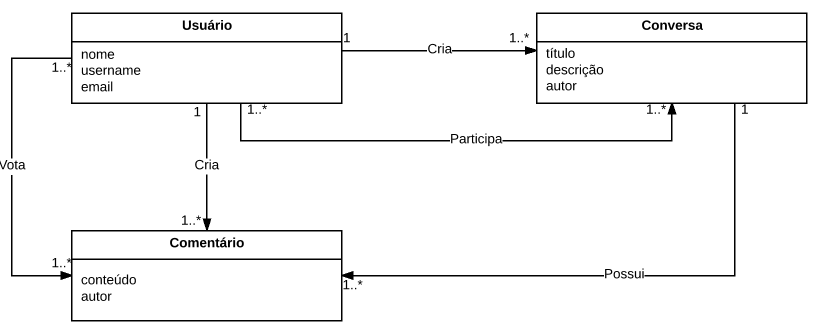
\includegraphics[scale=0.5]{figuras/entidades.png}
\caption{Entidades da API}
\label{fig:entidades}
\end{figure}

Considerando os requisitos funcionais e não funcionais da solução especificados anteriormente, a arquitetura da solução foi definida 
conforme a Figura \ref{fig:arquitetura_api}.

\begin{figure}[h!]
\centering
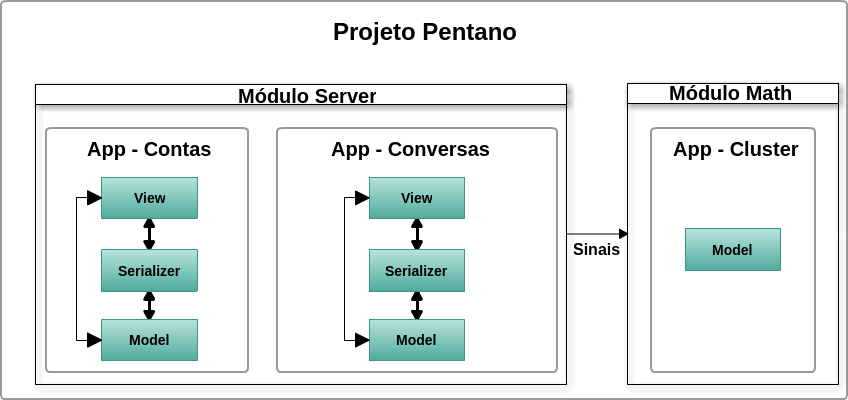
\includegraphics[scale=0.5]{figuras/arquitetura_api.png}
\caption{Entidades da API}
\label{fig:arquitetura_api}
\end{figure}

O módulo de serviço foi dividido em duas aplicações e ambas foram definidas em uma arquitetura
em 3 camadas: \textit{models}, \textit{views} e \textit{serializers}. 
A camada \textit{view} recebe e responde as requisições provenientes do cliente.
A camada \textit{serializer} é responsável pela leitura e conversão dos dados renderizados em JSON e os tipos e relações
definidas na aplicação.  

Por fim, a camada \textit{model} contém aspectos negociais relacionados a cada uma das entidades definidas na 
Figura \ref{fig:entidades}. Além disso, nessa camada é estabelecida a comunicação com o módulo de clusterização através de sinais.
Os sinais criados são disparados durante as requisições de realização de novos votos e o módulo de clusterização é registrado
como \textit{listener} desse evento.

Na Figura \ref{fig:resumo_ej_api} é apresentado o fluxo de funcionamento do ``Empurrando Juntos'' de acordo com a arquitetura
estabelecida para o Pentano.

\begin{figure}[bt!]
\centering
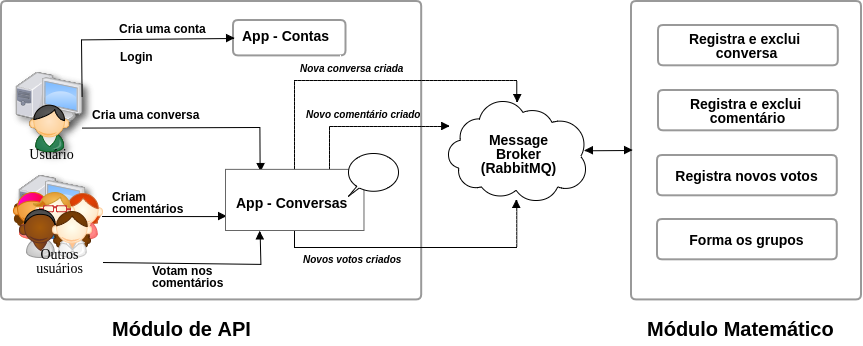
\includegraphics[scale=0.6]{figuras/resumo_ej_api.png}
\caption{Funcionamento do Empurrando Juntos - Comunicação entre os módulos}
\label{fig:resumo_ej_api}
\end{figure}

\vfill
\pagebreak

\section{Planejamento}

Para execução do trabalho foi realizado um planejamento que pode ser visto na Figura \ref{tab:planejamento}.
Foram contempladas as duas últimas etapas do trabalho, conforme definido no Capítulo \ref{cap:introducao}.
A etapa de Desenvolvimento da API será por meio de um processo iterativo e incremental com iterações de duas semanas. 

\begin{table}[h!]
\centering
\caption{Planejamento do trabalho}
\label{tab:planejamento}
\begin{tabular}{@{}cl@{}}
\toprule
\multicolumn{2}{c}{\textbf{Metas}}                                                                                                                         \\ \midrule
\multirow{3}{*}{Iteração 1}           & Estabelecimento da arquitetura                                                                                     \\
                                      & Implementação da feature de Gerenciamento de Usuário                                                               \\
                                      & Autenticação                                                                                                       \\ \midrule
\multirow{2}{*}{Iteração 2}           & Implementação da feature de Gerenciamento de Conversa                                                              \\
                                      & Implementação da feature de Gerenciamento de Comentário                                                            \\ \midrule
\multirow{2}{*}{Iteração 3}           & Implementação da feature de Agrupamento de usuários                                                                \\
                                      & Definição dinâmica da semântica dos votos                                                                          \\ \midrule
\multirow{2}{*}{Aplicação em um caso} & \begin{tabular}[c]{@{}l@{}}Estudo da adaptação da API para a temática de violência \\ contra a mulher\end{tabular} \\
                                      & Construção de um exemplo de uso da API                                                                             \\ \bottomrule
\end{tabular}
\end{table}

% \section{Resultados Esperados}








